
\section{Heaven}\label{sec:impl-intro}

The architecture of the \textsc{Test Stand} consists in three stand alone modules that establish a mono-directional communication flow: \textsc{Streamer}, \textsc{RSP Engine} and \textsc{Result Collector}. Some of the requirements reported in Section \ref{sec:requirements} directly affect the implementation experience of \name and Chapter \ref{chap:heaven} describes how fulfil them. First of all the requirements [R.10], i.e. the need of an \textit{Extendible Design}, and [R.11], which states the necessity of an \textit{Event-base architecture} to properly face any RSPEngine, are immediately relevant. 

To be \textit{Extendible} the \textsc{Test Stand} requires two main abstractions: the \textit{Event} and the \textit{EventProcessor}.

\textit{Event} concept is required to build a hierarchical communication. Indeed, the \textsc{Test Stand} may handle three events flows: one internal to the RSP Engine module, one for the communication between modules and one to communicate with the user. Next section about data clarifies the communication structured. 

The \textit{Event Processor} guarantees the system to be modular, it standardizes the interaction simplifying the behaviour of each component in the system. 

Thus, a module is an \textit{Event Processor} which can be positioned everywhere in the the \textsc{Test Stand} pipeline. % As a matter of facts, specific implementations of a module may reduce the generality of this definition and also the flexibility of the module itself.	

\begin{figure}[tbh]
  \centering
	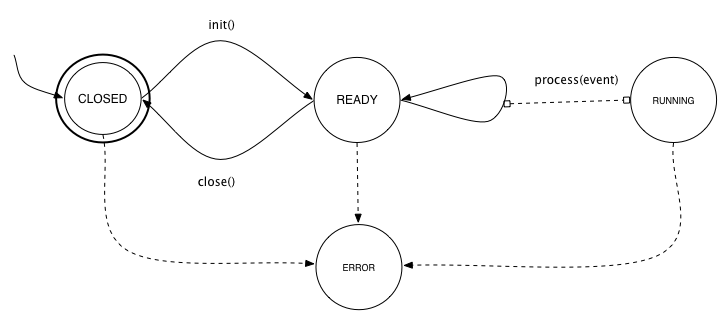
\includegraphics[width=\linewidth]{images/fsm-schema}
	\caption{Module Finite State Machine Automata} 
  	\label{fig:module-fsm}
\end{figure}

The requirement [R.4] states the \textsc{Test Stand} \textit{must not be running when the RSP Engine is under execution} (see Section \ref{sec:requirements}) conditioning \name workflow. To cover [R.4] we designed the status of each module  as a Finite State Machine (FSM), which can work only in those states that allow processing (READY). The schema in Figure \ref{fig:module-fsm} represents the FSM for each module of \name, even the Baselines, and also for the \textsc{Test Stand} external structure. 
A modules moves from CLOSED state to READY with a standard initialisation method. We state that each module is an \textit{EventProcessor} and the \textit{ process (Event e)} brings the module into RUNNING state until the processing ends, and then back to READY. One and only one module can be in the RUNNING state in a certain moment during the execution. This behaviour is exploited by the \textsc{Test Stand} external structure to control execution fulfilling [R.4] by stopping its process while the RSPEngine is running (see Section \ref{sec:teststand}). ERROR State, which can be reached from any point of the execution, prevents the propagation of errors over result data: when a module fails the execution is stopped without saving the erroneous data (last event) and reporting the error to the user.


\section{Events and Data}\label{sec:data-impl}

Chapter \ref{chap:problem-settings} poses the requirements of an Event-based architecture [R.11] for the \textsc{Test Stand}. Moreover, Chapter \ref{chap:heaven} describes \name workflow and how it exchanges events during the execution. The \textsc{Test Stand} modules interact trough events, see \ref{fig:uml_events},  which contains data at different points of the experiment process. \name handles three kind of events:

\begin{figure}[tbh]
  \centering
	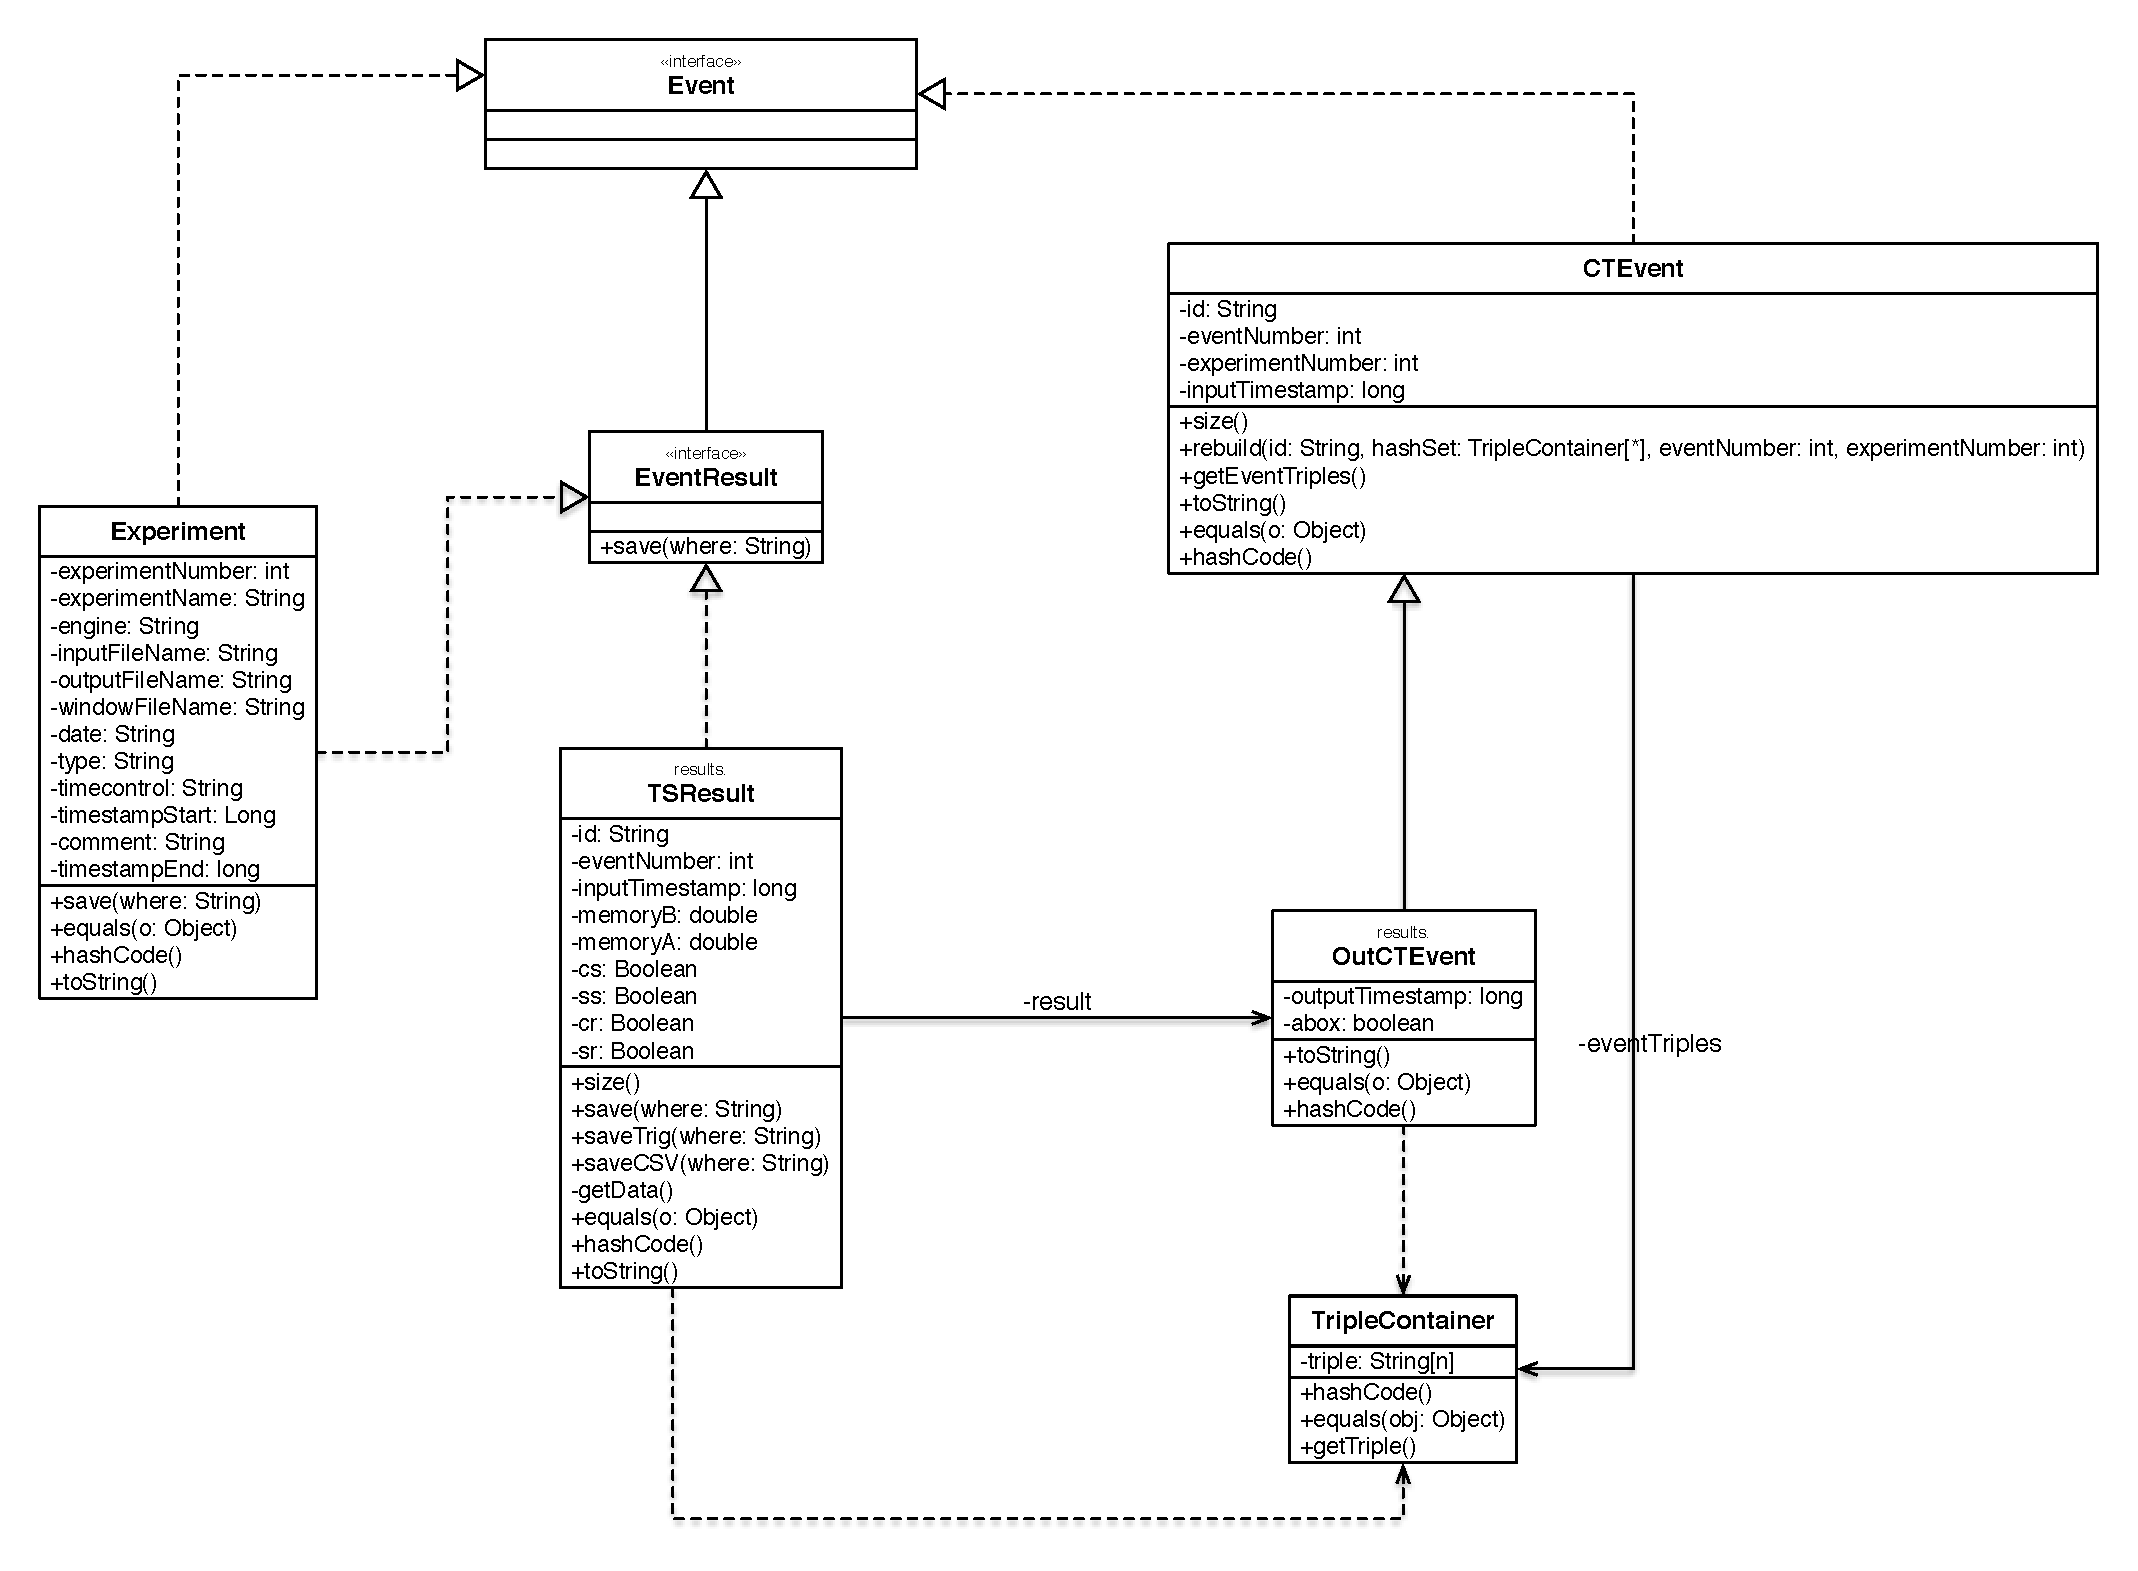
\includegraphics[width=\linewidth]{images/uml_events}
	\caption{UML Schema for all the events involved in the system} 
  	\label{fig:uml_events}
\end{figure}

\begin{itemize}
\item \textit{Experiment} - it represents the tuple $<\mathcal{E}, \mathcal{D},\mathcal{T},\mathcal{Q}>$ and all the experiment metadata like start time or end time.
\item \textit{CTEvent and OutCTEvent} - they contains a set of triples which has the same timestamp. The \textit{OutCTEvent} represents the event produced by the RSPEngine after processing the active window. Figure \ref{fig:uml_events} show the inheritance relation between \textit{CTEvent} and \textit{OutCTEvent}
\item \textit{TSResult} - it wraps the \textit{OutCTEvent} adding the information about the minimal sensor data: memory and latency and complete and soundness if it evaluated at runtime (see Section \ref{sec:requirements})
\end{itemize}

\name requires an initialization phase to prepare the \textit{Experiment} and provide it to the \textsc{Test Stand}. The current implementation exploits a property file with the Experiment parameters: ID and the tuple $<\mathcal{E}, \mathcal{D},\mathcal{T},\mathcal{Q}>$. 

The \textit{CTEvent} and the \textit{OutCTEvent} contain RDF triples in NT-Triple\footnote{http://www.w3.org/2001/sw/RDFCore/ntriples/}, which is the easiest RDF serialisation to parse. This serialisation was chosen to fulfil requirement [R.12], which demands an \textit{Easy-to-Parse RDF Serialisation for the events presented to the RSP Engine in exam}. Figure \ref{fig:uml_events} shows also that the RDF Triples are stored in the events into the \textit{TripleContainer} wrapper: we redefine the triple hashcode and equals method guaranteeing their uniqueness of within an \textit{CTEvent} or \textit{OutCTEvent}.

\section{Modules}\label{sec:modules-impl}

In Section \ref{sec:impl-intro} we define a module a an \textit{Event Processor} which can be positioned everywhere in the the \textsc{Test Stand} pipeline. Moreover, we introduce the FSM schema which describe a module lifecycle in \ref{fig:module-fsm}. We state that each module must be initialized to reach the READY state where the processing is allowed. 

The \textit{Startable} Interface standardize two methods, init() and close() which allow to control the behaviour of the Module at the start and the end of the execution. Notice that the ERROR state translate an exceptional behaviour which has to be handled exceptionally by each module, according with its internal mechanisms. 

In this section we present the three modules which compose \name: the \textsc{Streamer},  the \textsc{ResultCollector} and the  \textsc{Test Stand Supporting Structure}. They all extend the \textit{EventProcessor} concept and the \textit{Startable} interface, offering three standard method to interact with them: \textit{process(Event e)} from \textit{EventProcessor} and \textit{init()} and \textit{close()} from the \textit{Startable} Interface.

\subsection{Streamer}	\label{sec:streamer-impl}
\begin{figure}[tbh]
  \centering
	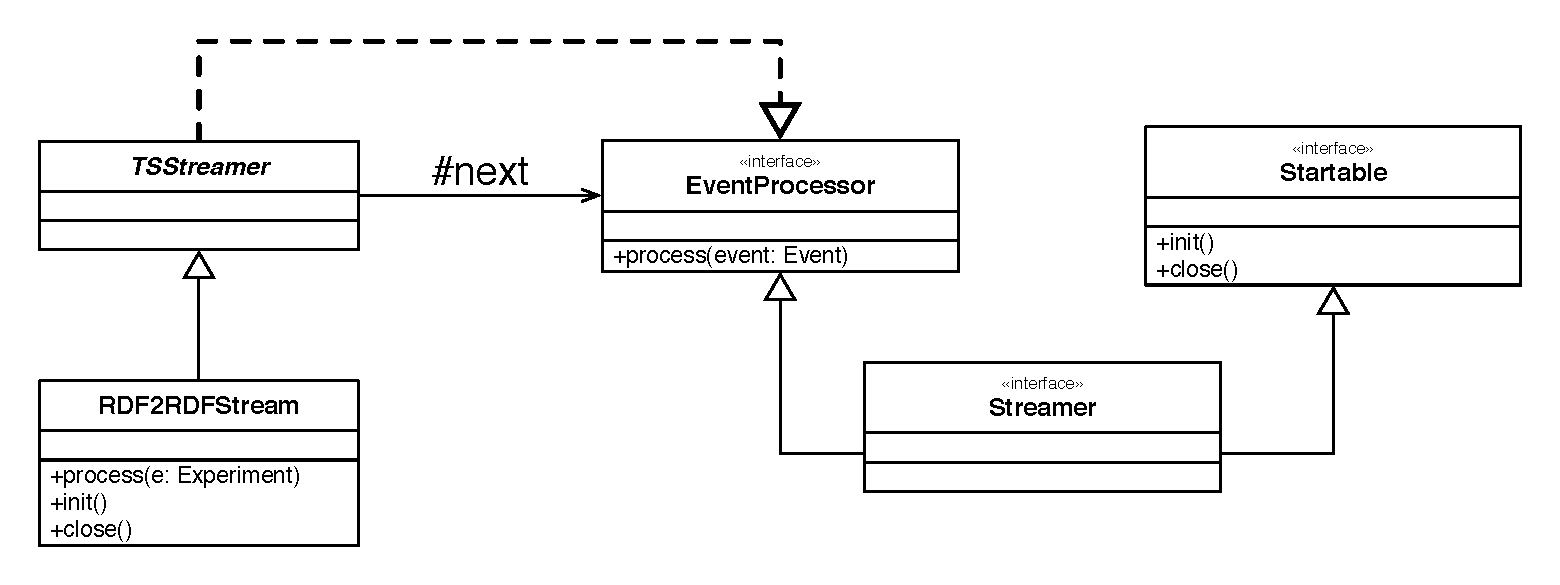
\includegraphics[width=\linewidth]{images/uml_tstreamer}
	\caption{Streamer UML Schema with TSStreamer and Implementation example} 
  	\label{fig:uml_tstreamer}
\end{figure}

The head-module in the \textsc{Test Stand} pipeline is the on \textit{TSStreamer}, see Figure \ref{fig:uml_tstreamer}, which is the most general implementation of the \textsc{Streamer}. The \textit{TSStreamer} processes an \textit{Experiment}, received by an external initialisation class. It and communicates, once initialized, with one referenced \textit{EventProcessor}, called \textit{next}, which process \textit{CTEvent} and follows in the pipeline. The nature of the communication between the\textit{TSStreamer} and the following \textit{EventProcessor} can follow the user needs, and passing different events. Notice that also the \textit{next} must be initialised before starting the communication, otherwise the ERROR state will be reached when the event is received by the \textit{next}, because the processing is not allowed.

Figure \ref{fig:uml_tstreamer} shows also the actual implementation, the \textit{RDF2RDFStream}, while in Figure \ref{fig:uml_flowrateprofiler} is presented its internal mechanism. 
The \textit{RDF2RDFStream} was developed to conduct experiments as they are presented in Chapter \ref{chap:evaluation}.  It is worth to note that we use LUBM Benchmarks to generate the data for the experiments. LUBM generated data are static, thus the \textit{RDF2RDFStream} builds an RDFStream attaching to the static data produced by LUBM a timestamp. The file is generated using  LUBM(1000,0), which means 1000 different universities with the random generation seed 0. 

\begin{figure}[tbh]
  \centering
	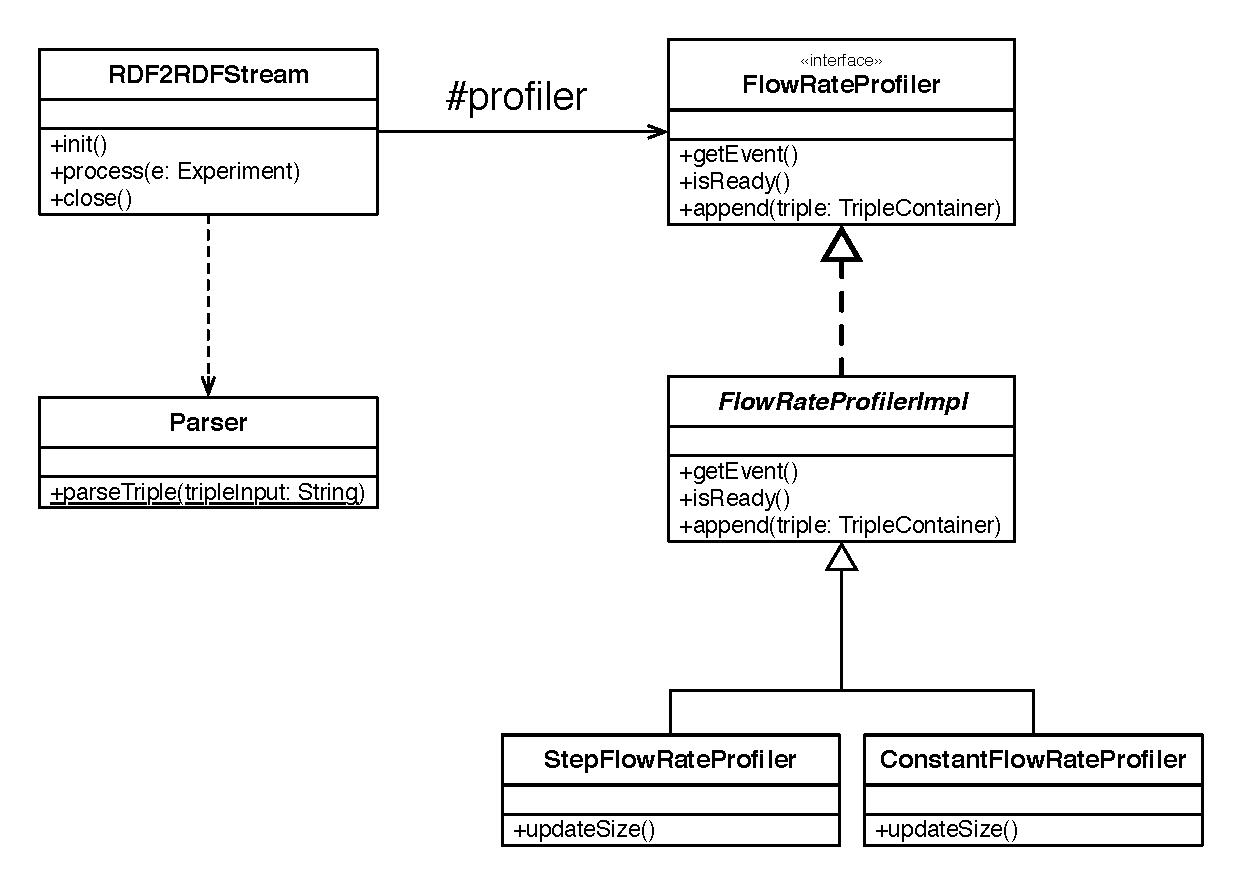
\includegraphics[width=0.75\linewidth]{images/uml_flowrateprofiler}
	\caption{RDF2RDFStream internal UML Schema} 
  	\label{fig:uml_flowrateprofiler}
\end{figure}


The \textit{Parser} component, in Figure \ref{fig:uml_flowrateprofiler} can be accessed statically by \name modules. It reads in memory one by one the triples in the file guaranteeing data independence [R.1] and it does not influence the memory footprint [R.5] by allocating only the memory necessary to parse a triple. 

Figure \ref{fig:uml_flowrateprofiler} also includes the \textit{FlowRateProfiler}. This component determines the number of triples to add to a \textit{CTEvent} and builds such an event. In this way, \textit{RDF2RDFStream} can generate different RDF streams $\mathcal{D}$, which differ on the number of contemporary triples in the stream. 

\begin{figure}[tbh]
\centering
\subfigure[Exponential Growing Size: $y=2^x$]{
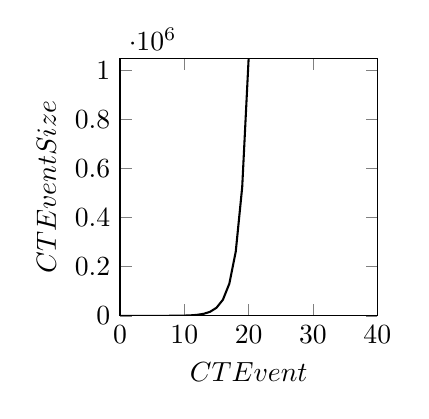
\begin{tikzpicture}
  \begin{axis}[ 
  width=0.4\linewidth,
      height=0.4\textwidth,
    xlabel=$CTEvent$,
    ylabel={$CTEvent Size$},
    xmin=0.00, xmax=40,
	ymin=0, ymax=1048576
  ] 
    \addplot [
    line width=0.75pt]
    coordinates {
    		(0.00, 1.00)
		(1.00, 2.00)
		(2.00, 4.00)
		(3.00, 8.00)
		(4.00, 16.00)
		(5.00, 32.00)
		(6.00, 64.00)
		(7.00, 128.00)
		(8.00, 256.00)
		(9.00, 512.00)
		(10.00, 1024.00)
		(11.00, 2048.00)
		(12.00, 4096.00)
		(13.00, 8192.00)
		(14.00, 16384.00)
		(15.00, 32768.00)
		(16.00, 65536.00)
		(17.00, 131072.00)
		(18.00, 262144.00)
		(19.00, 524288.00)
		(20.00, 1048576.00)
		};	
		
	\end{axis}
\normalsize

\end{tikzpicture}
}
\subfigure[Step Growing Size with K1=100 and K2=1000 after 9 CTEvents]{
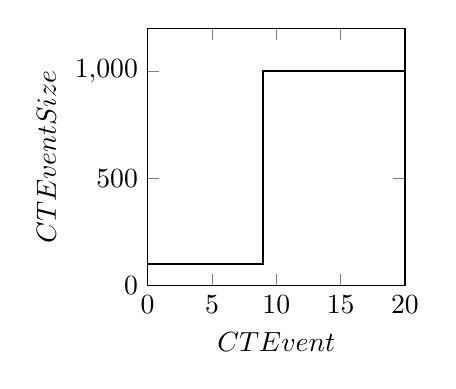
\begin{tikzpicture}
  \begin{axis}[ 
  width=0.4\linewidth,
      height=0.4\textwidth,
    xlabel=$CTEvent$,
    ylabel={$CTEvent Size$},
    xmin=0.00, xmax=20,
	ymin=0, ymax=1200
  ] 
    \addplot [
    line width=0.75pt]
    coordinates {
    		(0.00, 100.00)
		(1.00, 100.00)
		(2.00, 100.00)
		(3.00, 100.00)
		(4.00, 100.00)
		(5.00, 100.00)
		(6.00, 100.00)
		(7.00, 100.00)
		(8.00, 100.00)
		(9.00, 100.00)
		(9.00, 1000.00)
		(10.00, 1000.00)
		(11.00, 1000.00)
		(12.00, 1000.00)
		(13.00, 1000.00)
		(14.00, 1000.00)
		(15.00, 1000.00)
		(16.00, 1000.00)
		(17.00, 1000.00)
		(18.00, 1000.00)
		(19.00, 1000.00)
		(20.00, 1000.00)
		};	
		
	\end{axis}
\normalsize

\end{tikzpicture}
}
\caption{Example of CTEvent size growing by the FlowRateProfiler}
\label{fig:frp-examples}
\end{figure}


The \textit{FlowRateProfiler} builds the triple according to a function $y=f(x)$, in which $x$ is the number of the \textit{CTEvent} and it results that $y$ is the number of triple this \textit{CTEvent} will contain. 

Practically $f$ can be any function from N to N. For example if we decide to increase linearly the number of triples inside a \textit{CTEvent} the function $f$ will be: \[y=x, \text{ where } x,y \in N\]

The first event (E0) will contain zero triple, E1 will contain only one triple following E4 will contain four triples and so forth. Another possibility is to increase exponentially the number of triples inside a \textit{CTEvent} : \[y=2^x, \text{ where } x,y \in N\] 
The first event (E0) will contain one triple, E1 will contain two triple following E3 will contain eight triples and so forth, Figure \ref{fig:frp-examples}.a shows the resulting behaviour plotting the triple number on y-axis and \textit{CTEvent} number on x-axis

We develop two \textit{FlowRateProfiler} for our experiment: 
\begin{itemize}
\item \textit{ConstantFlowRateProfiler}, which maintains the same number of triples for each events over all the experiment: \\
\[y=K, \text{ where } K \in N \]

\item \textit{StepFlowRateProfiler}  which maintain a constant number of triple $K1$ inside a \textit{CTEvents} for $x$ events, specified in the set-up phase. When $x$ are created,  suddenly changes the number of triple $y$ form $K1$ to $K2$ where $K2 >> K1$. Figure \ref{fig:frp-examples}.b contains the resulting plot of implemented function which follows:

\[
y=
\begin{cases}
K1, &\text{if $x < M$ } $ where $ K1, M \in N\\
K2, &\text{if $x >= M$} $ where $ K2 >> K1, K2 \in N
\end{cases}
\]


\end{itemize}
Other implementations are available in \name right now, but are not used in the experiments:
\begin{itemize}
\item \textit{LinearStepFlowRateProfile}, which stream $x$ CTEvents of dimension $y$, in terms of triples, then linearly increase the number of a quantity $M$: \[y=x*M, \text{ where } x,y,M \in N\]
\item \textit{ConstantRandomFlowRateProfiler}, which changes $y$ and $x$ according with two random generators directed by two seeds. \[y=random(seed), \text{ where } random(seed),y \in N\]
\end{itemize}


\subsection{Result Collector} 

\noindent The \textsc{ResultCollector} is the acquisition system that collects the query results and the measurements data gathered by the \textsc{Test Stand} during the execution of an experiment.

\begin{figure}[tbh]
  \centering
	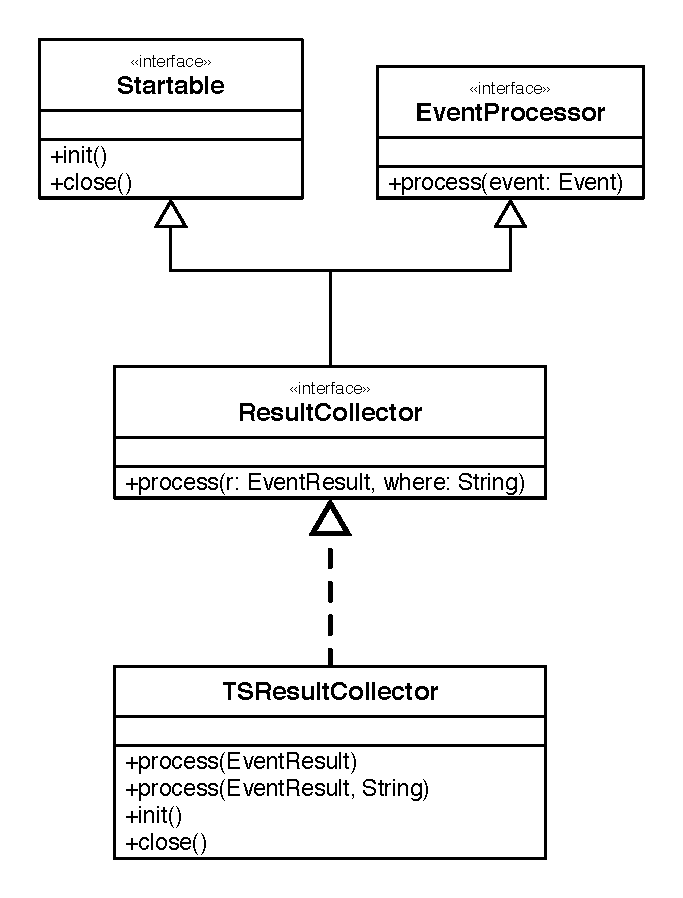
\includegraphics[width=\linewidth]{images/uml_resultcollector}
	\caption{ResultCollector UML Schema with events Experiment, TSResult and OutCTEvent} 
  	\label{fig:uml_resultcollector}
\end{figure}

The UML Schema in Figure \ref{fig:uml_resultcollector} shows the implementation of the \textit{ResultCollector} interface, named \textit{TSResultCollector}, which is again an \textit{EventProcessor}. The \textit{TSResultCollector} stays at the end position in the pipeline which composes the \textsc{Test Stand}. It is responsible of saving data in a way that is independent from which data format, since requirement [R.7] demands to \textit{enable users extensions with new software sensors and specific measurements collection}.  The general saving procedure exploits the \textit{EventResult} interface, which exposes methods to delegate the implementation of such a procedure to the provider of the event, according to his needs. Figure \ref{fig:uml_resultcollector} shows the relation between the \textit{EventResult} interface and the \textit{TSResultCollector}, which calls the exposed methods \textit{save(location)} over all the events passed to it during the execution. 


\begin{figure}[tbh]
  \centering
	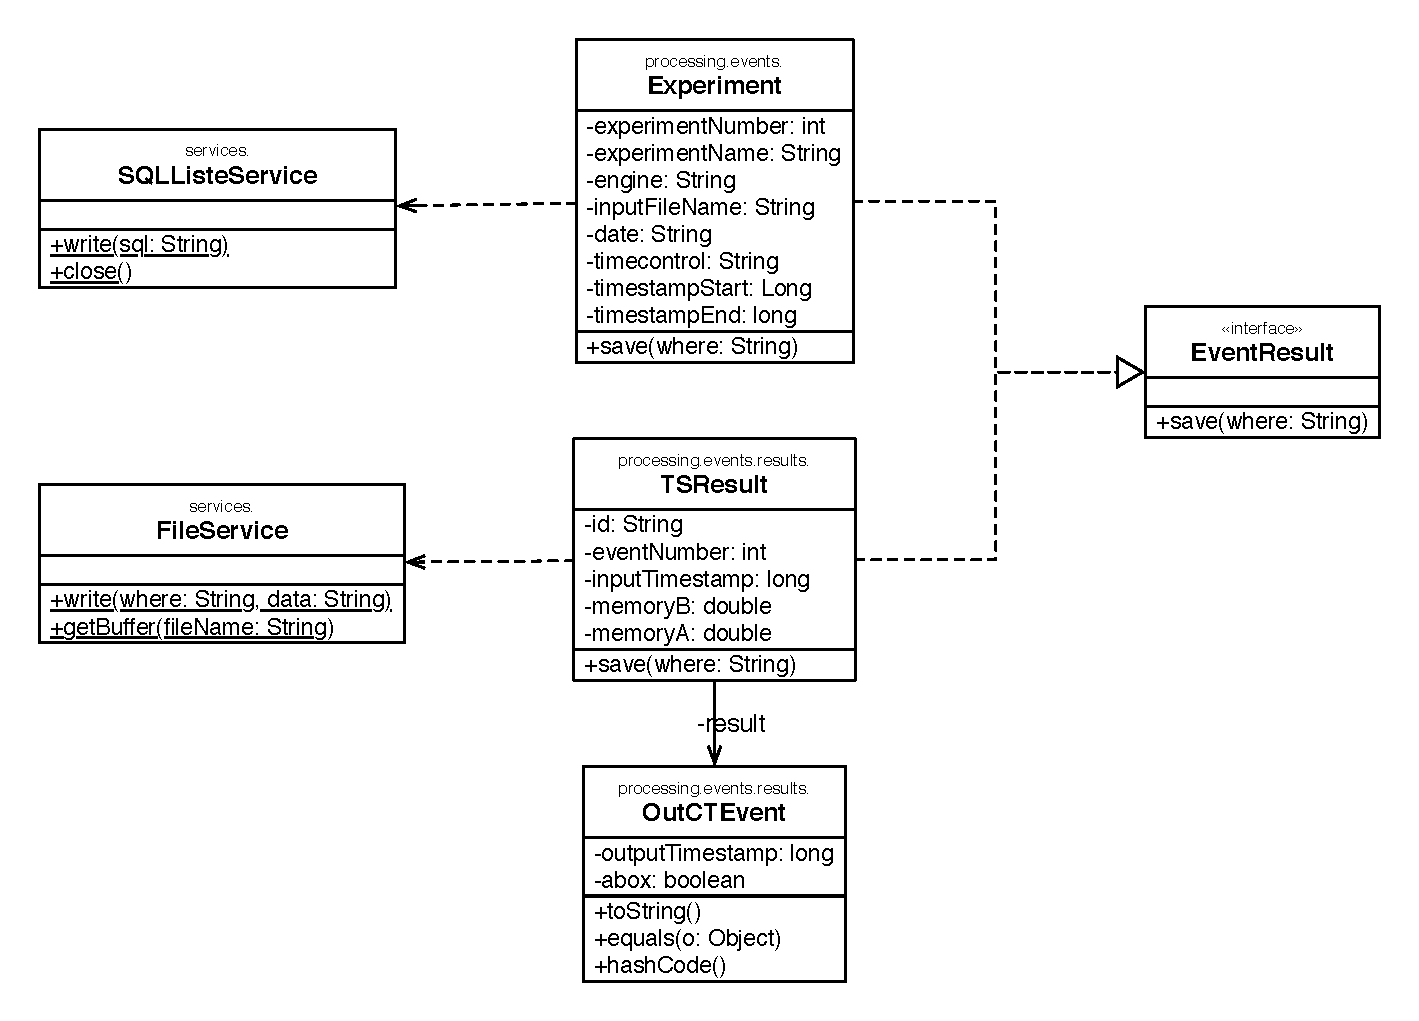
\includegraphics[width=\linewidth]{images/uml_resultcollector_events}
	\caption{ResultCollector events  UML Schema: Experiment, TSResult and OutCTEvent} 
  	\label{fig:uml_resultcollector_events}
\end{figure}

Moreover, Figure \ref{fig:uml_resultcollector_events}, shows how different events in the system exploit the \textit{EventResult} interface. In the current implementation the \textit{TSResultCollector} handles two kinds of event:
\begin{itemize}
\item \textit{TSResult} - it saves the data of the query results into a TriG\footnote{http://www.w3.org/TR/trig/} file where the graph name is the event id inside the experiment, while it save the sensor data with event id into a CSV\footnote{$http://en.wikipedia.org/wiki/Comma-separated_values$} file. 
\item \textit{Experiment}. It saves the experiment metadata and the tuple \\ $<\mathcal{E},\mathcal{D},\mathcal{T},\mathcal{Q}>$ collapsed into a generic description field into SQLite\footnote{https://sqlite.org/} database.
\end{itemize} 

The two saving procedure exploits service classes, the \textit{SQLLIsteService} and the \textit{FileService} in Figure \ref{fig:uml_resultcollector_events}, which exposes static methods to interact with the file-system. The goal is  reducing system complexity offering a single point to interact with the file-system, which usually is a slow operation, to avoid parallel interactions that may influence the experiment. 


\subsection{Test Stand Supporting Structure}\label{sec:teststand-impl}


\begin{figure}[tbh]
  \centering
	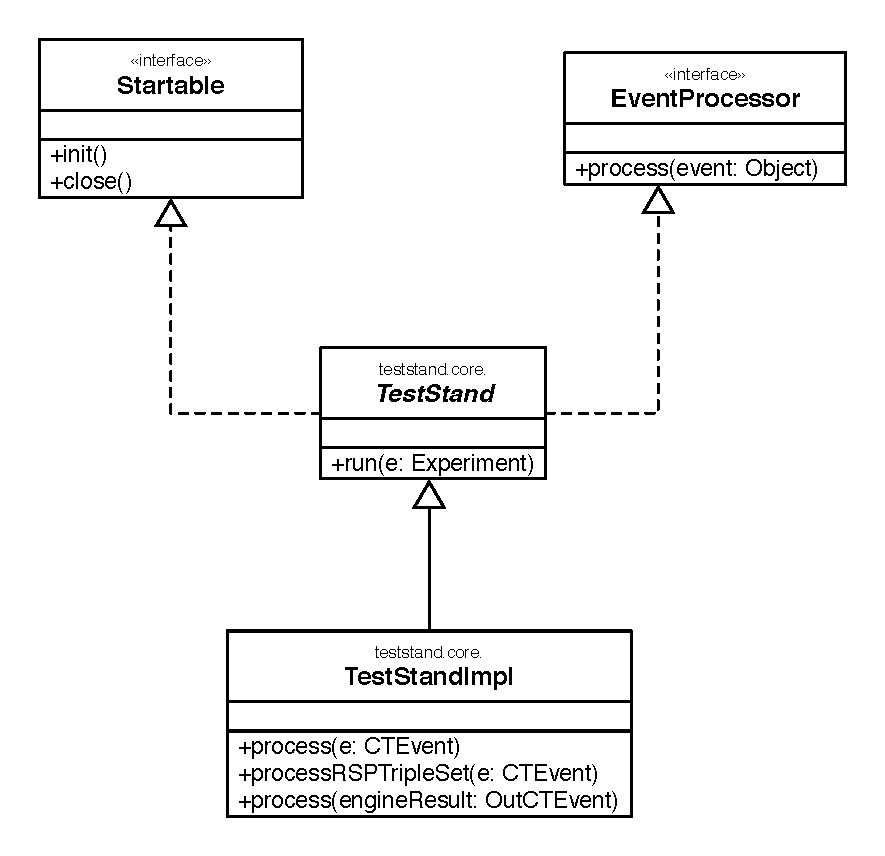
\includegraphics[width=\linewidth]{images/uml_teststand}
	\caption{UML Schema the TestStand} 
  	\label{fig:uml_teststand}
\end{figure}


\name \textsc{Test Stand} was defined as set of modules which interact exchanging events during the execution. However, Chapter \ref{chap:heaven} describes at the design level the presence of an external structure which orchestrates the communication between the \textsc{Streamer}, the \textsc{RSP Engine} and the \textsc{ResultCollector}. This external structure also exposes the APIs for users interaction. Figure \ref{fig:uml_teststand} shows both these classes called \textit{TestStand} and its current implementation is the \textit{TestStandImpl}.


Figure \ref{fig:uml_teststand} shows that the \textit{TestStand} structure is and \textit{EventProcessor} as other modules. The relation between the \textit{TestStand} and other modules is presented in Figure \ref{fig:uml_teststand_modules}. The \textit{TSStreamer}, the \textit{RSPEngine} and the \textit{TSResulCollector} are linked to the \textit{TestStandImpl} trough an initialisation class which receives the configuration file, and sets these modules up according with the requirements [R.1] for data independence  [R.2] and [R.3] for engine independence and query independence. Once the set-up phase is complete the \textit{TestStandImpl} is initialized1 and it consequently initialises all the upstanding modules. The \textit{Experiment} is created externally and passed to the \textit{TestStandImpl} to start the execution. 

\begin{figure}[tbh]
  \centering
	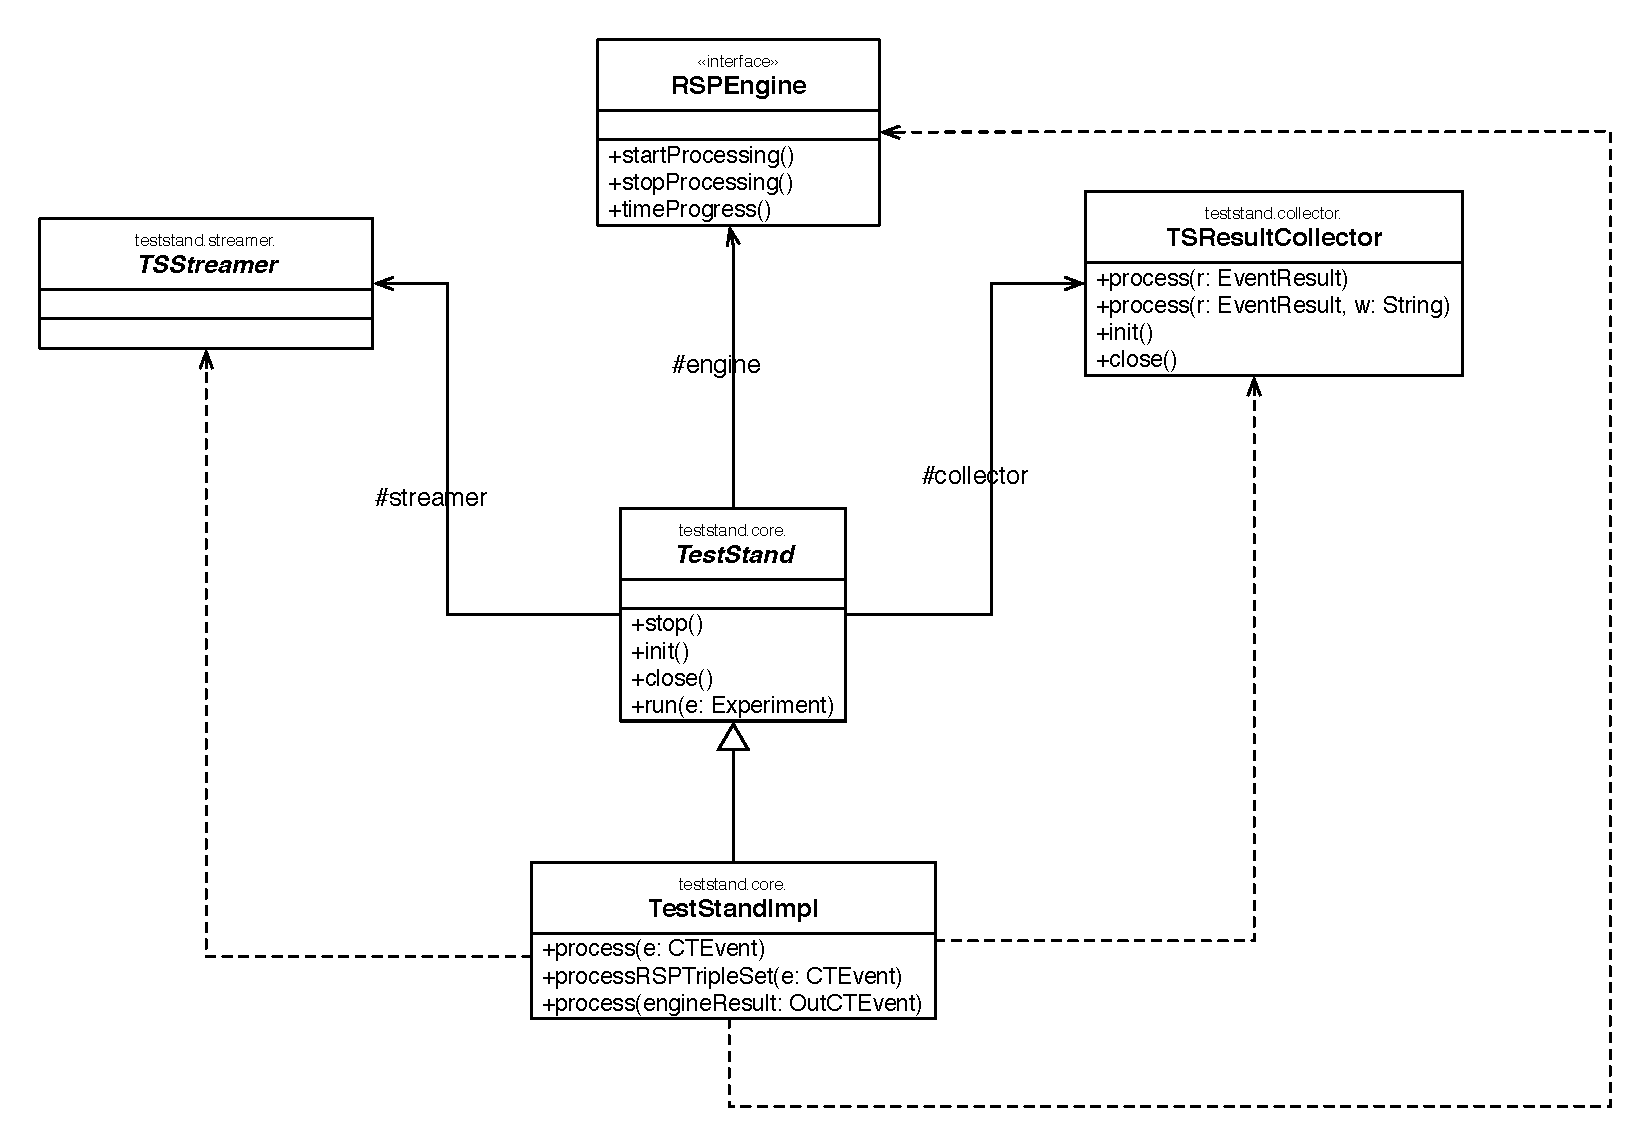
\includegraphics[width=0.90\linewidth]{images/uml_teststand_modules}
	\caption{UML Schema the TestStand with the upstanding modules: TSStreamer, RSPEngine, TSResultCollector} 
  	\label{fig:uml_teststand_modules}
\end{figure}

During the execution \textit{TestStandImpl} intercepts the \textit{CTEvents} form the \textit{TSStreamer} and sends them to the \textit{RSPEngine} as described in Section \ref{sec:arch-workflow}. According with the \textit{Experiment} specification the \textit{TestStandImpl} turns off or on its sensors. It calculates latency starting a timer when the \textit{CTEvent} arrives and stops the timer when it \textit{RSPEngine} outputs the results. It retrieves the memory usage asking the JVM in both the point above [R.6]. To fulfil requirements [R.7] any new measurement can take place  when the \textit{RSPEngine} is not running yet or when it has finished the computation. Once the \textit{OutCTEvents} comes form the \textit{RSPEngine}, the \textit{TestStandImpl} receives it and wraps it within a \textit{TSResult}, then it sends the query results data together with the measures to the \textit{TSResultCollector} fulfilling [R.8] and supporting [R.9] for further analysis with the Analyser.
%
%R.6 include basic set of performance measurements [?].
%R.7 enable users extensions with new software sensors and specific measure-
%ments collection.
%R.8 support performance measurements collection for further analysis.

\section{Baselines}\label{sec:baselines-impl}

\name Baselines are four elementary implementations of an RSP Engine which follow the design proposal presented in Section \ref{sec:baselines}, covering [R.13]. They pipeline Esper\footnote{$http://www.espertech.com/esper/$}, a mature commercial DSMS, with the Jena general purpose rule engine\footnote{http://jena.apache.org/documentation/inference/\#rules
}, a flexible reasoning engine. The aim of the choice of Esper and Jena is fulfilling requirement [R.14], baselines Eligibility, coupling this two good solutions for stream processing and reasoning, to obtain a fair solution in the SR context. 

\begin{figure}[tbh]
  \centering
	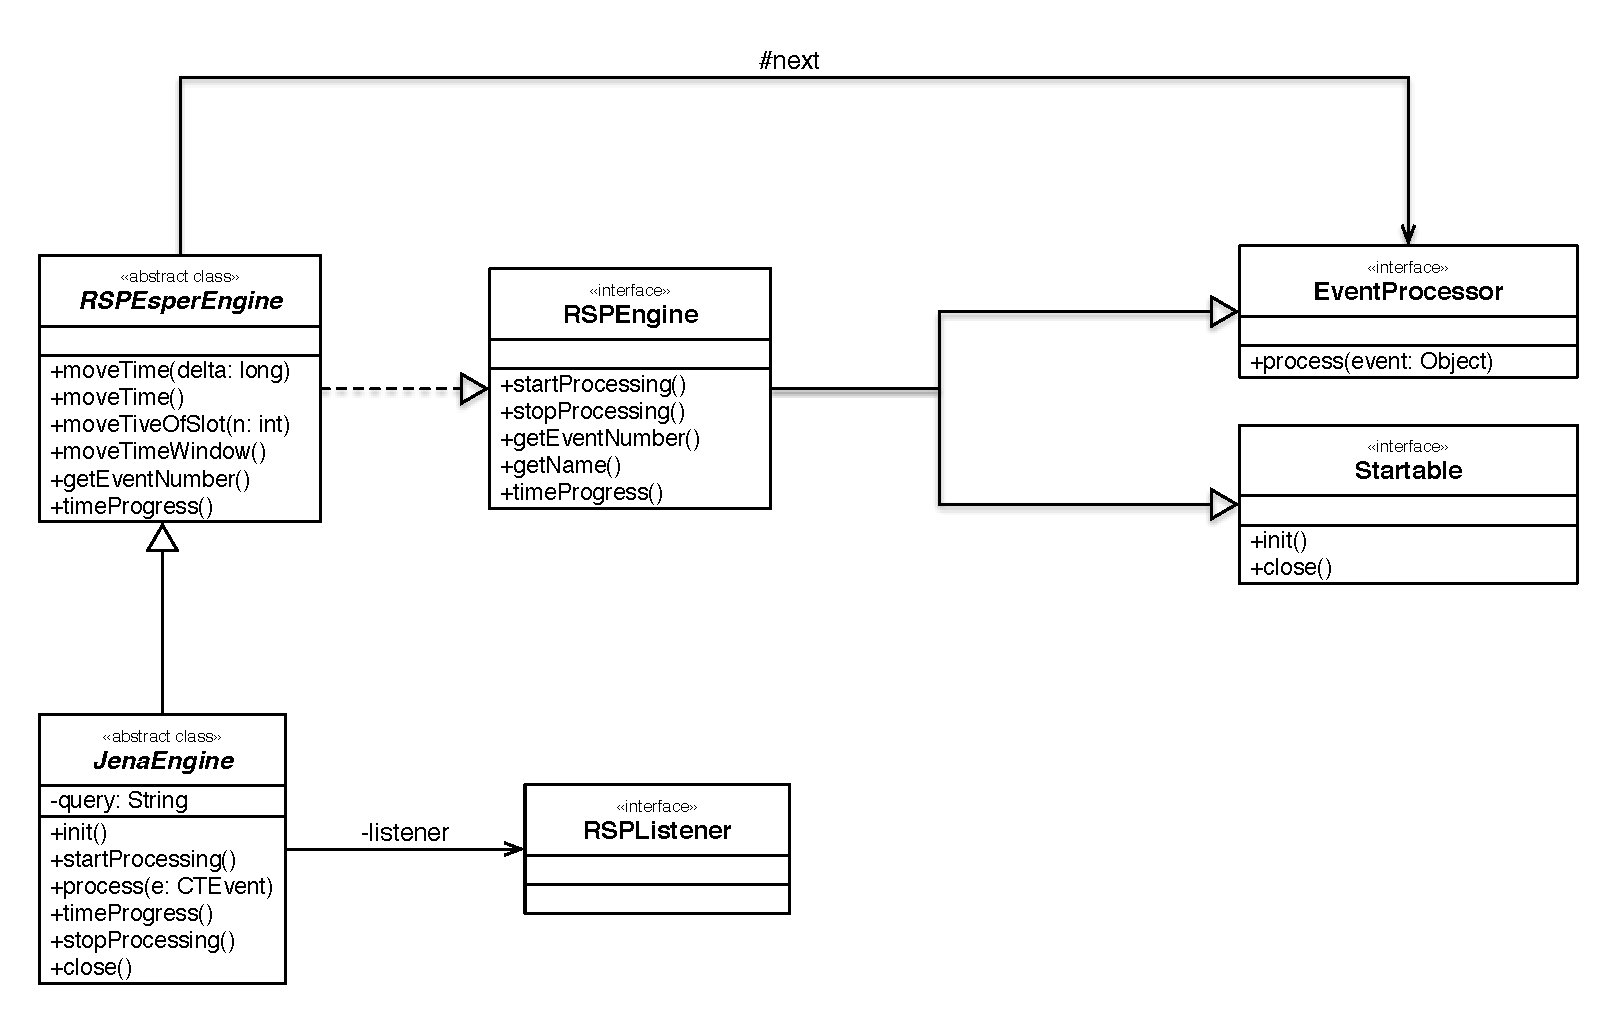
\includegraphics[width=\linewidth]{images/uml_baselines_general}
	\caption{RSPEsper Engine General UML Schema} 
  	\label{fig:uml_baselines_general}
\end{figure}

In Figure \ref{fig:uml_baselines_general} is presented how the baselines are implemented. The general structure exploits the \textit{RSPEngine} interface, a proxy for the \textit{EventProcessor} and the \textit{Startable}  interfaces described in Section \ref{sec:impl-intro} and in Section \ref{sec:modules-impl}. 

All the proposed baselines take advantage of the ability of Esper to be temporally controlled by an external agent\footnote{\url{http://esper.sourceforge.net/esper-0.7.5/doc/reference/en/html_single/index.html#api-controlling-time}} by sending time-keeping events to synchronise the internal time flow. The \textit{RSPEsperEngine} abstract class implements the \textit{RSPEngine} interface in order to share the Esper runtime definition for all the baselines. 

To enable external time control the \textit{RSPEngine} interface exposes the \textit{moveTime()} method, whose implementation depends on the particular RSP Engine in use; in this case of the method is implemented by the \textit{RSPEsperEngine} encapsulating the logic to send a time-keeping event into Esper: one time-keeping event is sent before injecting the triples within a \textsc{CTEvent} and another one after all triples in \textsc{CTEvent} were sent. In this way all the triples in the \textsc{CTEvent} are consider contemporary by the baselines. 

The \textit{RSPEsperEngine} contains also the reference to an \textit{EventProcessor}, called \textit{next}, which represents the module which follows the RSP Engine in the \textsc{Test Stand} pipeline. The next \textit{module} can be any modules which processes \textit{CTEvent}. In the current implementation the \textit{Test Stand External Structure } follows the RSP Engine, to intercept the outcoming \textit{OUTCTEvents}.

\begin{figure}[tbh]
  \centering
	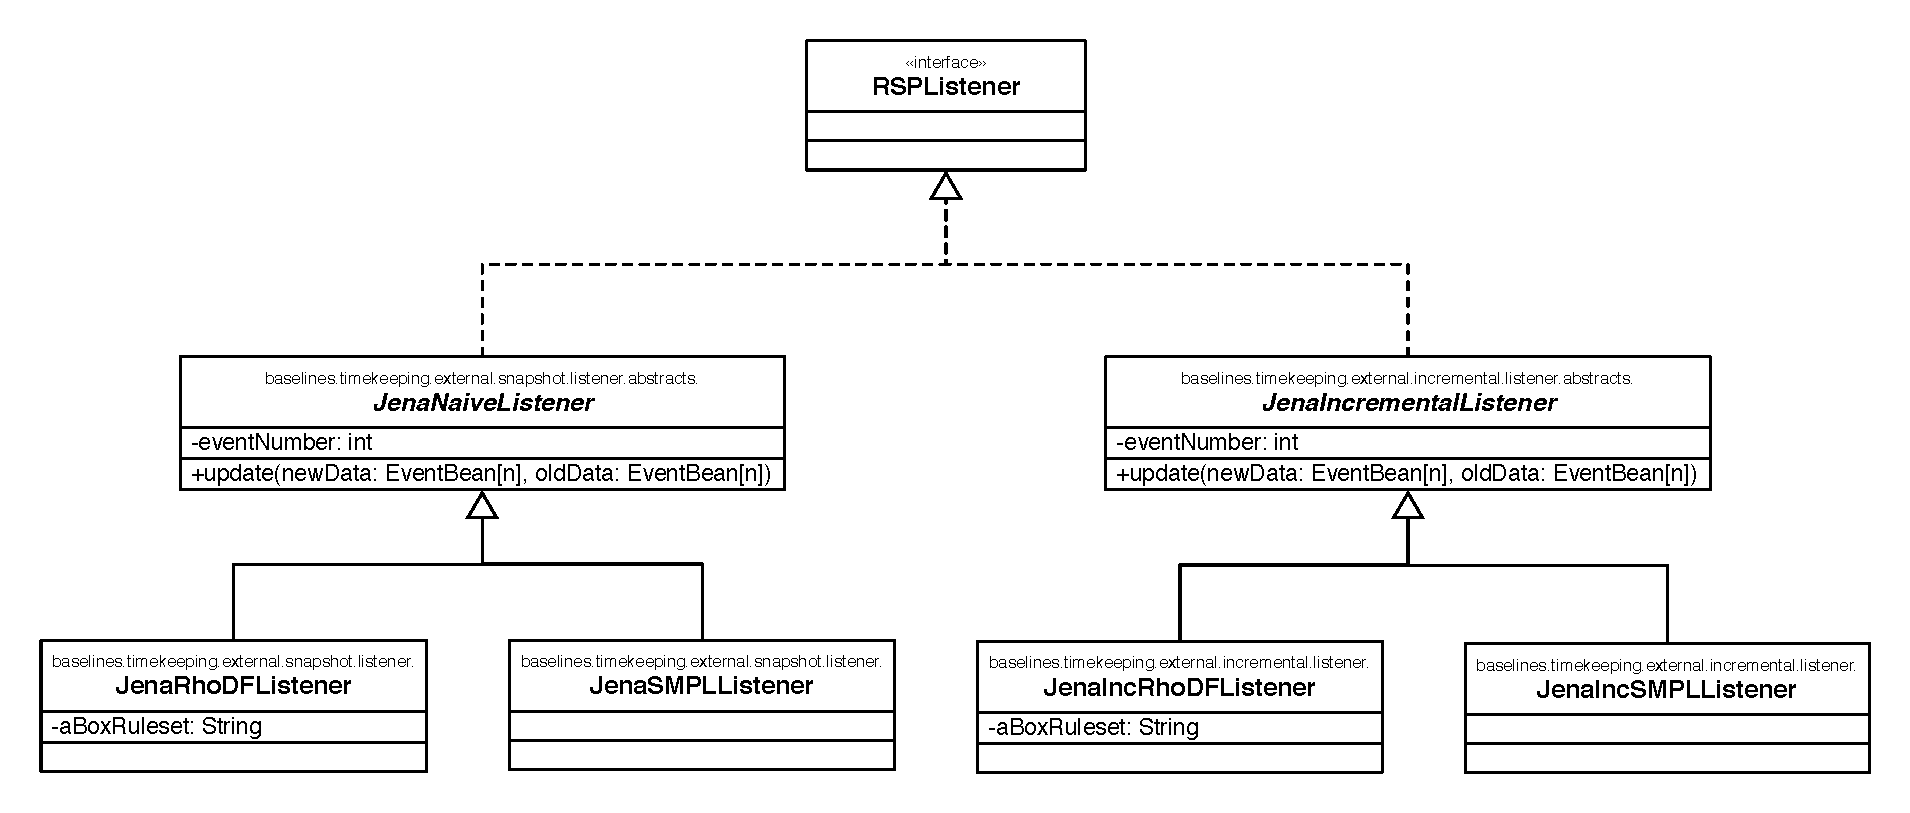
\includegraphics[width=\linewidth]{images/uml_baselines_listener}
	\caption{RSPListener UML Schema} 
  	\label{fig:uml_baselines_listener}
\end{figure}

The \textit{JenaEngine} abstract class in Figure \ref{fig:uml_baselines_general} represents the general implementation of a baseline. It allows to design the processing delegating the engine specification to  the \textit{RSPListener} class, which as  Figure \ref{fig:uml_baselines_listener} shows, is responsible to pipeline the Jena rule engine to the DSMS. Moreover, the figure includes the different implementation the listener, which variates the reasoning approaches, Naive or Incremental, as demanded by [R.15] (baseline relevance) and according to the baseline design presented in Section \ref{sec:baselines}. Neither the \textit{JenaNaiveListener} or the \textit{JenaIncrementalListener} specify the entailment regime, which must be defined with specific implementations as it is visible again in the Figure \ref{fig:uml_baselines_listener}.

\begin{figure}[tbh]
  \centering
	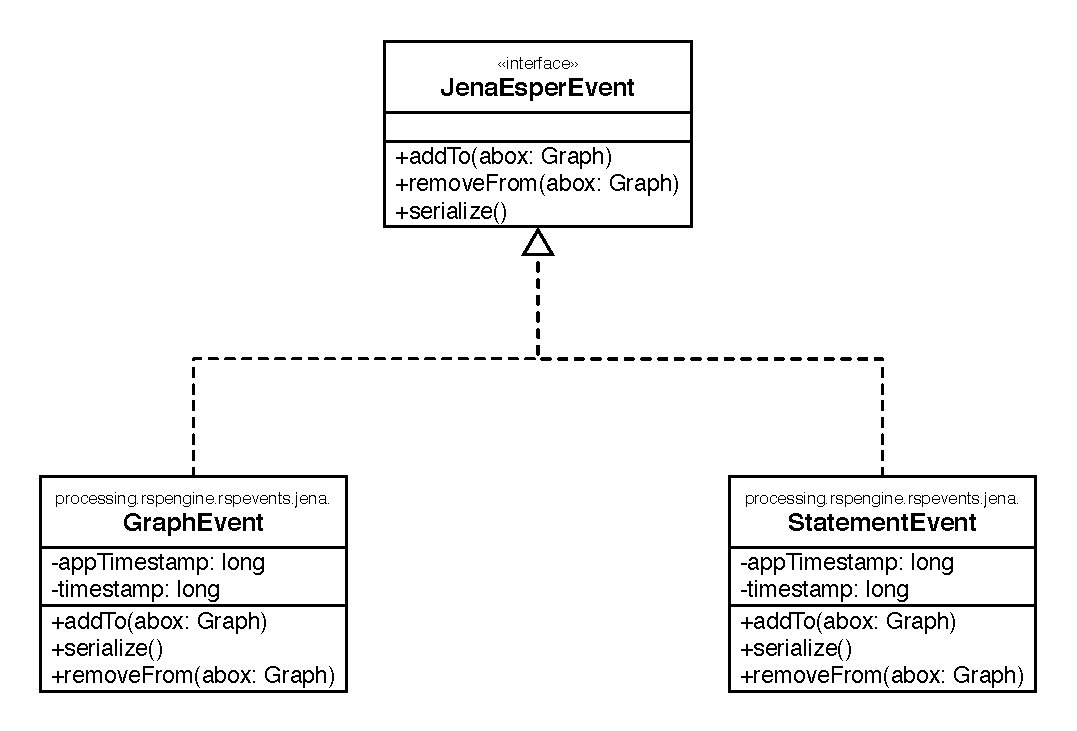
\includegraphics[width=0.8\linewidth]{images/uml_baselines_events}
	\caption{Esper-level events UML Schema} 
  	\label{fig:uml_baselines_events}
\end{figure}

The baselines relevance demanded by [R.15] comes also from the different implementation of the RDFStream model, Graph Based or Triple Based, which for Esper-based RSP engine depends on which events are registered to Esper runtime. Figure \ref{fig:uml_baselines_events} shows that all events exposed the same methods to interact with the RDF model, provided by the \textit{JenaEsperEvent} interface. 

Notice that when a \textit{CTEvents} comes to the RSP Engine it will be transformed into the events handled by the DSMS, contained in Figure \ref{fig:uml_baselines_events}. This translation process influences the latency calculus, because the time spent by the engine to translate events from the RDFStream into its internal mechanism may be relevant. Once the processing is complete, the output of the RSP Engine is injected into an \textit{OUTCTEvent} and passed to the next \textit{EventProcessor} in the pipeline, which is the \textsc{Test Stand}, also the translation time for producing the output is part of the engine response time.


\begin{figure}[tbh]
  \centering
	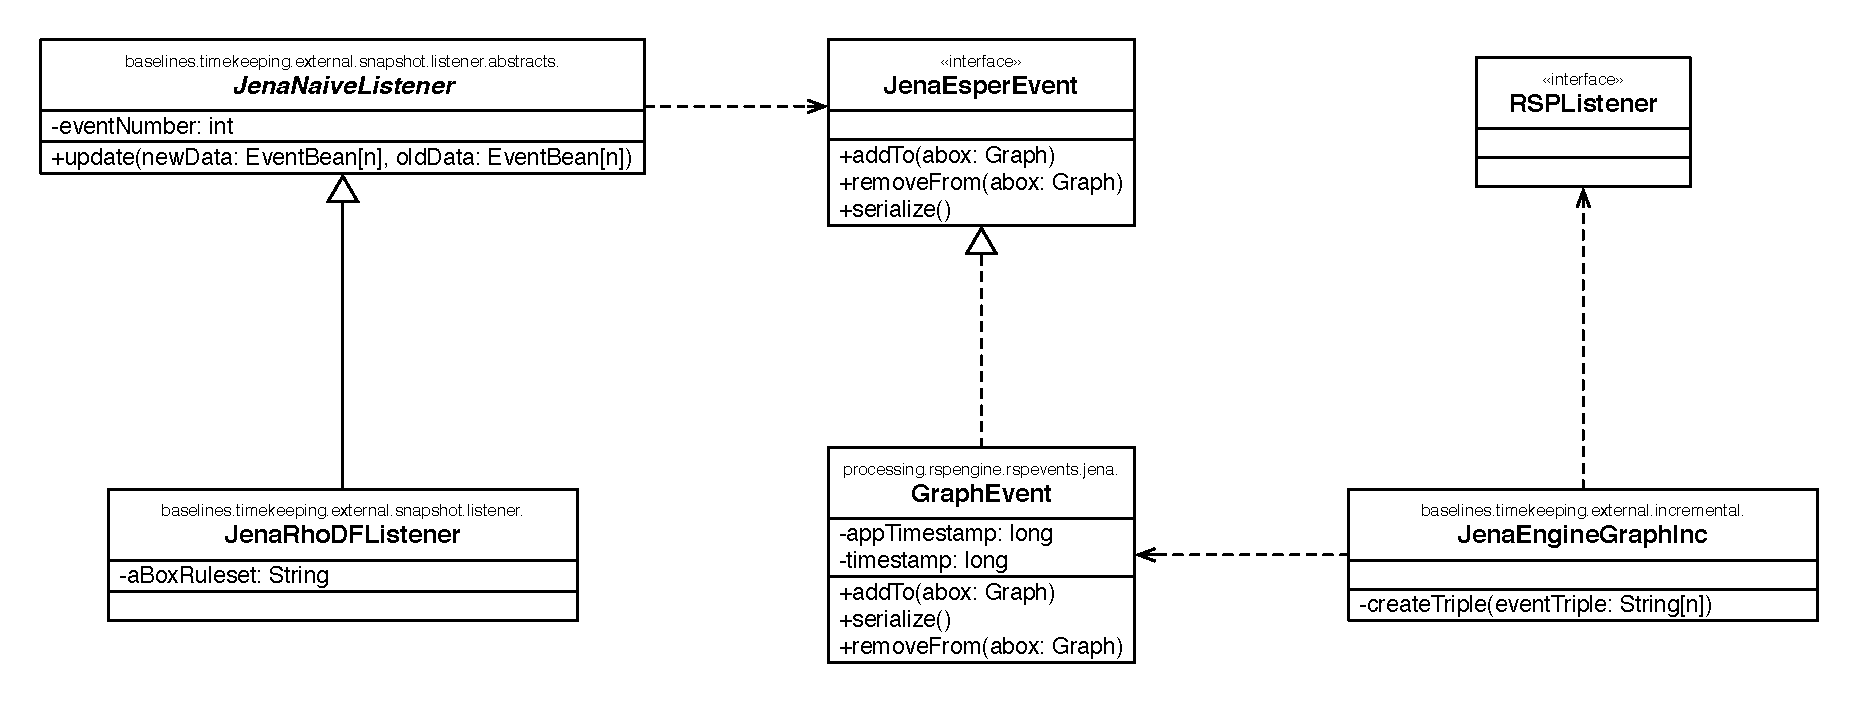
\includegraphics[width=\linewidth]{images/uml_baselines_rel_listener_event}
	\caption{RSPListener and events UML Schema} 
  	\label{fig:uml_baselines_rel_listener_event}
\end{figure}

\textit{JenaNaiveListener} and the  \textit{JenaIncrementalListener} handle the events which come form the DSMS trough the \textit{JenaEsperEvent} interface, Figure \ref{fig:uml_baselines_rel_listener_event} report  the structure for the case of Graph-based event representation (see Section \ref{sec:baselines} for event details). 

This levelled stricture of  baselines code allow to share the majority of the code by splitting the different architectural elements. In this way we fulfil [R.16] which demands baseline Simplicity.


\section{Analyser}\label{sec:analyser-impl}

\begin{figure}[tbh]
  \centering
	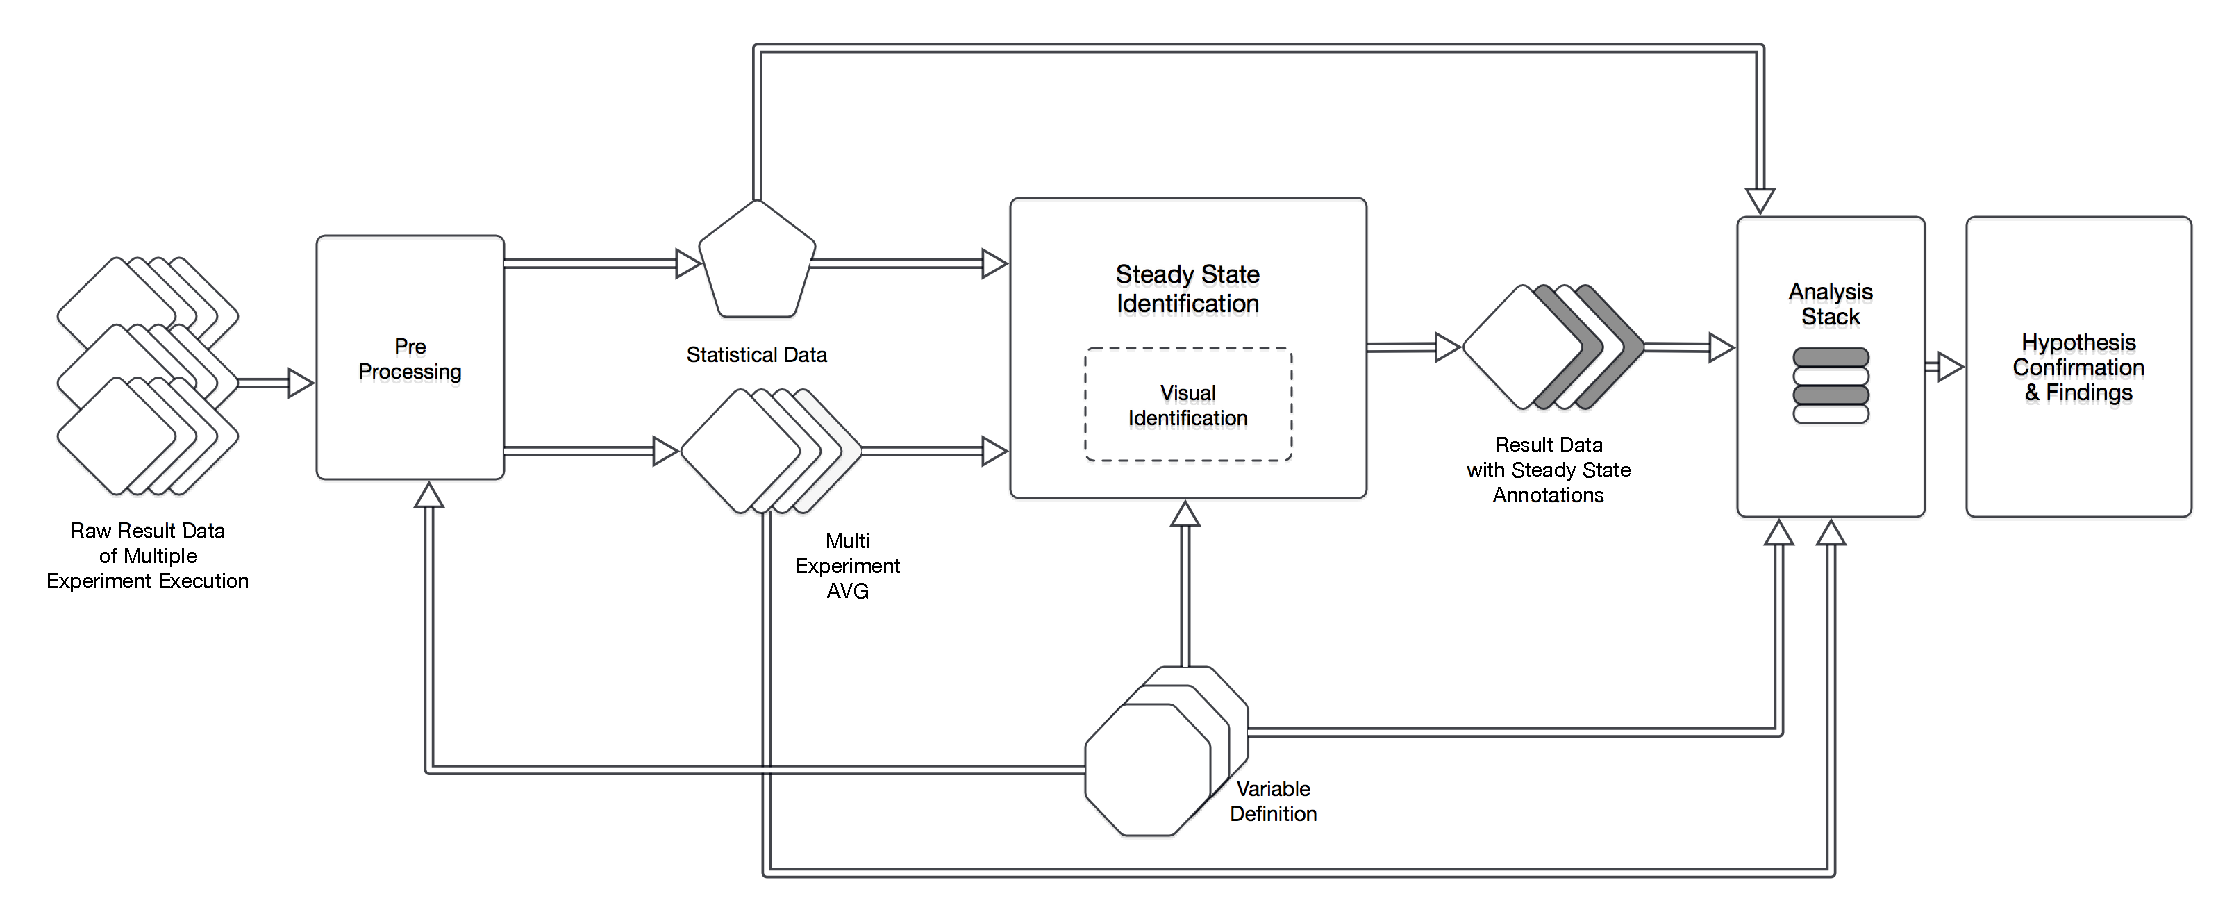
\includegraphics[width=\linewidth]{images/analyser-block-schema-impl}
	\caption{Analyser Blocking Schema: Implementation Detail Level} 
  	\label{fig:analyser-block-schema-impl}
\end{figure}

In Section \ref{sec:analyser} we introduce the \textsc{Analyser} as set of methods for data processing and analysing, which allow to refute or confirm hypothesis and improve existing models trough empirical findings. Moreover, we draw in Figure \ref{fig:analyser-block-schema} the block schema of the \textsc{Analyser}, reported in Figure \ref{fig:analyser-block-schema-impl} detailing the each level of the analysis block.

In this section we describe how the different block are implemented, which analysis are possible and which tools sustain each level of analysis.
Notice that the relation between the hypothesis and tools to apply the analysis is deep and hard it is hard to generalise the investigation. The first one depends on the the research question, while the second one requires to study the data, which are related to the experiment.  However, it is possible to identify some common characteristics that have a general meaning. Independently from the hypothesis and  experiment we can consider the tools to sustain the investigation methods. Indeed, they apply the Systematic Comparative Approach presented in Chapter \ref{chap:problem-settings}), which demands to identify characteristics upon which is possible to build comparison. 

First of all, the \textsc{Analyser} receives two input: the raw data form the experiments and the variables to build the analysis, \ref{fig:analyser-block-schema-impl}. Both the Steady State Identification block and Analysis Block require an automatic procedure,named pre-processing, which averages the data of multiple executions of the same experiment. Even if the Test Stand is designed to be system independent, it is a dynamic system as the ones we want to study. Strange results may happen while an experiment is running. In order to reduce and possible eliminate the outliers, multiple runs of the same experiment must be mediated obtaining the average measures. 


Once we have reliable data, the Steady State Identification Block can process them and evidence, w.r.t the evaluated variable, it a solution has reached the Steady State condition for a certain variable. Automatic procedures to identify the State State condition exist, but they require dedicated studies which will be faced as future works. At this moment Steady State Identification exploit data visualisation and is it no automated. Visualise the point of when Steady State is reached is necessary to exclude the initial warm-up period form the data and properly verify hypothesis. Anyhow, we know that the graphical method is limited, it must be applied for each system variable, because they may reach the equilibrium at different times.


In the Analysis Block we can decline the comparative research approach either to the visual analysis or statistical investigation, trough the different levels presented in \ref{sec:analyser}. The graphical analysis method is more qualitative then the second one, but reading the information presented in graphical way can be preferred in those case where numerical data are not clear. On the other hand, the statistical investigation method demands more complex instruments to interpret the data, but allows to answer also elaborate questions with simpler answers. Following we present for all the Analysis level the method involved in the current implementation.

\pagebreak


\textsc{Level 0 - Dashboards}

\begin{figure}[tbh]
  \centering
	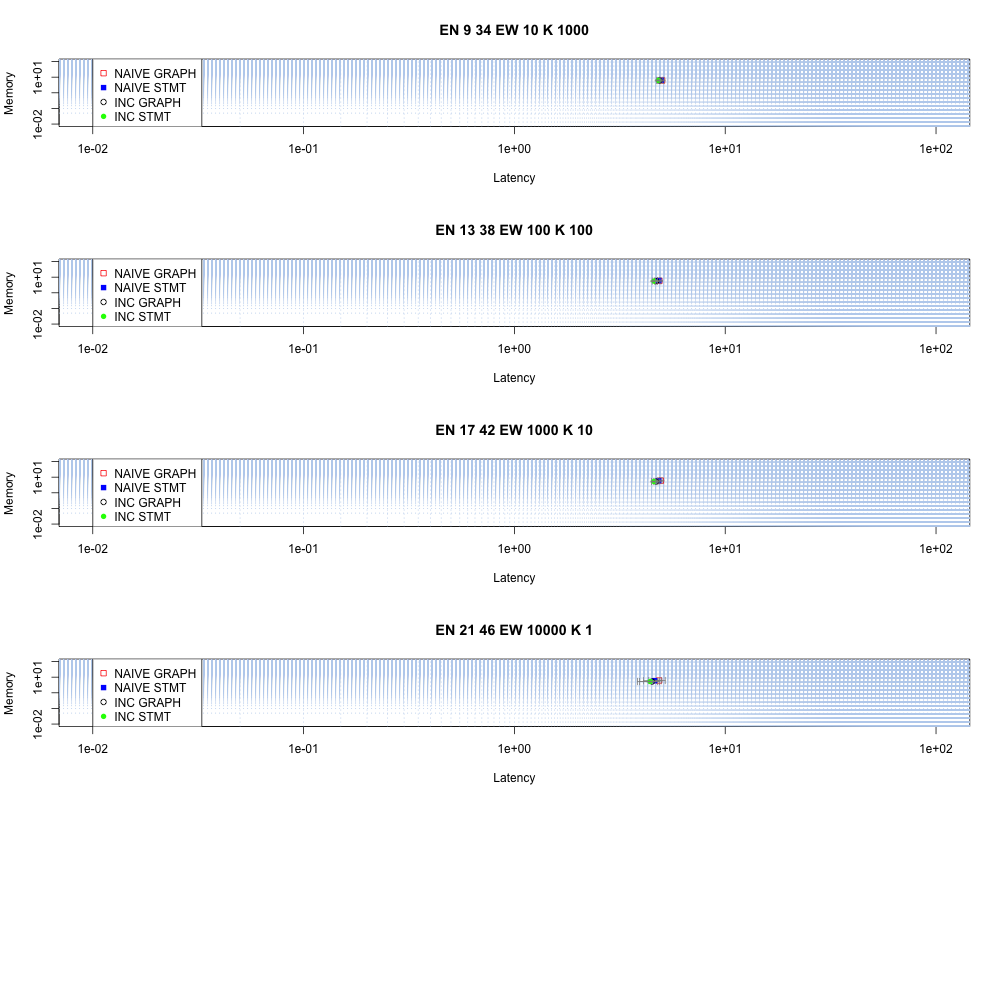
\includegraphics[width=0.45\linewidth]{images/dashboard-example}
	\caption{Example of Dashboard Representation} 
  	\label{fig:dashboard-example}
\end{figure}


Figure \ref{fig:dashboard-example} contains an example of the possible Dashboard representation. The aim of dashboard like the one in Figure \ref{fig:dashboard-example} is to represent the multiple solution in a n-variable space. This kind of representation allow to define the solution dominance w.r.t the involved variable, stating which solution, if any, is better then another one within an experiment or which experimental setting dominates the other for a given RSP Engine.\\

\textsc{Level 1 -  Statistical Values Comparison}\\

\begin{table}[htb]
\scriptsize
	\centering
	\subtable[Symbolic Comparison of variables A vs B on Experiment 1]{%
		\begin{tabular}{c | cccc} % creating eight columns
	  	\hline
		A vs B & \multicolumn{4}{c}{Experiment 1 Condition A}  \\
		 Comparison  & &&&\\
		\hline
		   	        & $\simeq$\\
		 Experiment 1 & A     & 	$\simeq$  & A & B\\
		 Condition  & A     & 	$\simeq$  & $\simeq$ & B\\
		 B          & A     & 	$\simeq$  & B & A\\
		\hline % inserts single-line
	 \end{tabular}
	}\qquad\qquad
	\subtable[Symbolic Comparison of variables A vs B on Experiment 1]{%
		\begin{tabular}{c | cccc} % creating eight columns
	  	\hline
		A vs B & \multicolumn{4}{c}{Experiment 1 Condition A}  \\
		 Comparison  & &&&\\
		\hline
		   	        & $\simeq$\\
		 Experiment 1 & 10\%     & 	$\simeq$  & 42\% & 33\%\\
		 Condition  & 23\%     & 	$\simeq$  & $\simeq$ & 12\%\\
		 B          & 20\%    & 	$\simeq$  & 22\% & 22\%\\
		\hline % inserts single-line
	 \end{tabular}
	}
	\caption{(a) symbolic-comparison over two variables - (b) numeric-comparison over a common variable }
	\label{tab:comp-tables}
\end{table}

Time series describe how a dynamic system evolves over time, so it is meaningful to attempt hypothesis verification trough statistical values, which always consider the the Steady State to allow the generalisation of the insights. The most common metrics are average and standard deviation and maximum or minimum for a certain variable. 
Tables \ref{tab:comp-tables} (a) and (b) show two example of statistical analysis at different detail levels. Table \ref{tab:comp-tables}.a contains the symbolic comparison of two solution over a given variable.  Table \ref{tab:comp-tables}.b offers a deeper details level, showing how much a solution is better than the other. How to choose the proper level depends on the needs of the research. 

Moreover, trough this disposition of experiment result is possible to move in tables cell, changing the experimental setting. It is easy to understand how different experiment influence the behaviour of an RSP Engine: moving on the horizontal axis of Table \ref{tab:comp-tables}.a we can variate the Condition A appreciating the differences. Actually this kind of analysis is generated into a CSV report, which contains all the meaningful statistical values for the experiments. The report can be further manipulated to obtain the table visualisation. \\

\textsc{Level 2 - Patter Identification}\\

\begin{figure}[tbh]
  \centering
  \subfigure[Pattern Recognition Example: Memory in Frequency Domain]{
  	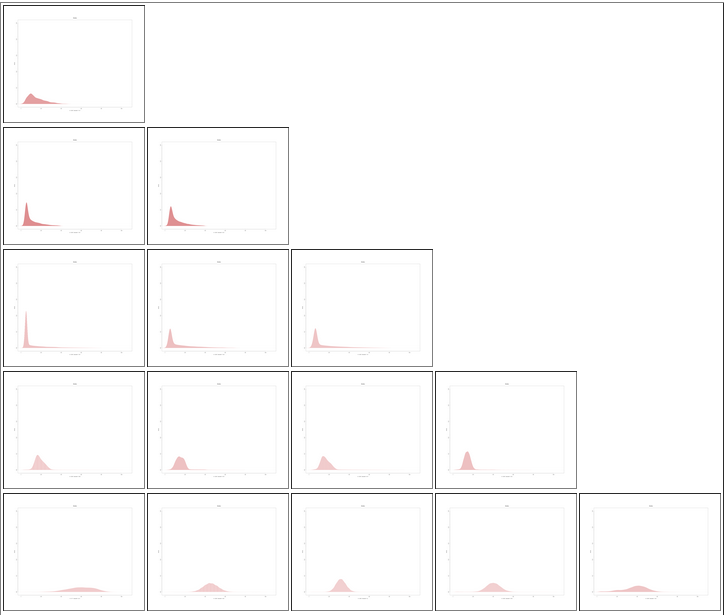
\includegraphics[width=0.45\linewidth]{images/pattern-example-density}
  	
  }
  \subfigure[Pattern Recognition Example: Memory in Time Domain]{
  	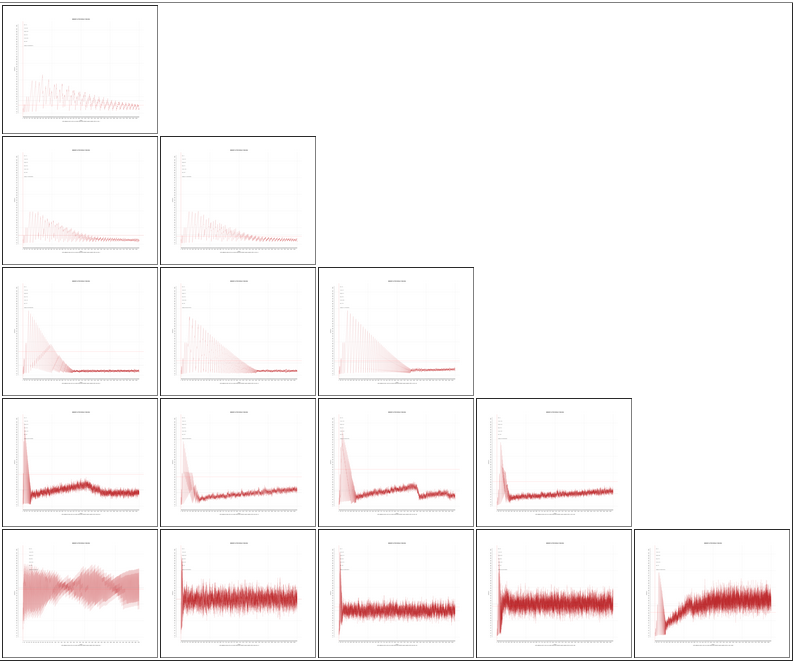
\includegraphics[width=0.45\linewidth]{images/pattern-example-memory}
  }
	
	\caption{Two Examples of Pattern Recognition} 
  	\label{fig:pattern-examples}
\end{figure}

Figure \ref{fig:pattern-examples} (a) and (b) exploit the same experiment representation used in Table \ref{tab:comp-tables} of Level 2. Trough this disposition is possible to identify graphical pattern. This level comparisons allow to appreciate together multiple experiments results, for a given variable (memory in this case). 

Moving up and down in Figure \ref{fig:pattern-examples}.a for example is possible to understand how memory distribution is influenced by changing the variable on the vertical axes. The same observation can be done moving from the left to the right or cross tables diagonals. Ordering experiment like in Figure \ref{fig:pattern-examples} provides a new a global view over multiple experiments.\\

\textsc{Level 3 - Visual Comparison}\\

\begin{figure}[tbh]
  \centering
  \subfigure[Multi-Experiment Comparison]{
  			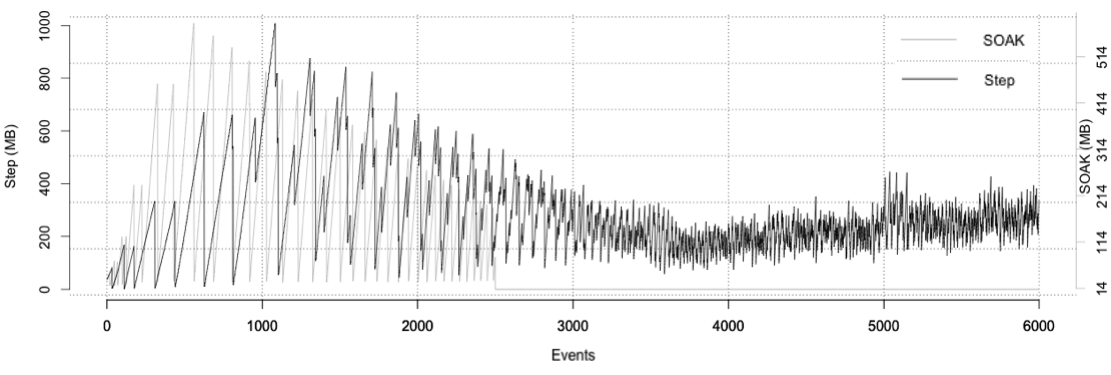
\includegraphics[width=0.80\linewidth]{images/comp-inter}
  			}
  \subfigure[Multi-Variables Comparison]{
  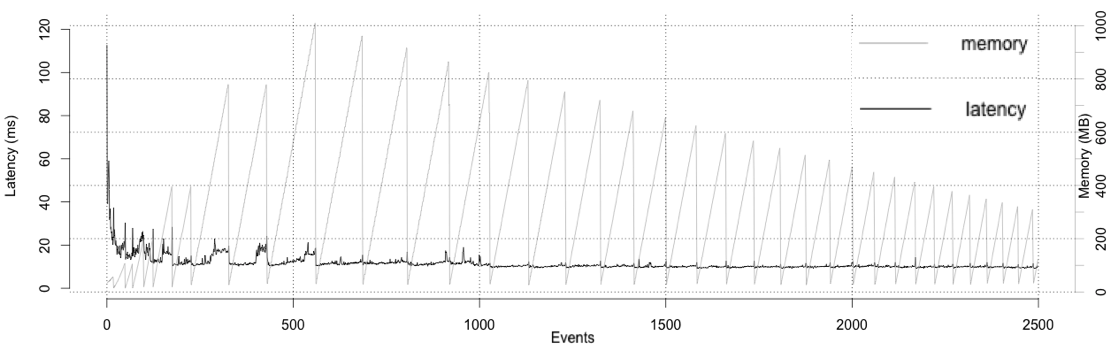
\includegraphics[width=0.80\linewidth]{images/comp-intra}
  }
  \caption{Visual Comparison} 
  \label{fig:visual-comp}
\end{figure}

Finally, the lowest level of analysis focuses on single graphical visualisation. Figure \ref{fig:visual-comp} contains two possible analysis. Plotting multiple variables over the same chart allow to better understand the relation, for example if one reaches the Steady State before the other as happens for Latency w.r.t Memory in Figure \ref{fig:visual-comp}.b. Comparing different experiment over the same variable allow similar observation too, focusing on the relation between the experimental settings. In summary:

\begin{enumerate}
\item[A] Figure \ref{fig:visual-comp}.a shows an example of inter-experiment investigation: multi-plotting the same variable, arguing about the similarity or the difference upon different experiments. 
\item[B] Figure \ref{fig:visual-comp}.b shows an example of intra-experiment investigation, multi-plotting the different variables within the same experiment; 

\end{enumerate}


%Time series studies usually start with data visualisation analysis. The most common plotting tools represent the series in temporal form. Moreover, it is relevant to visualise their behaviour in the frequency domain. 
%Independently from the Steady State condition, variables relation can be evidenced in a comparative form and the Analyser must support this kind of studies. We distinguish three main investigation options, the following images show a some examples of them:
%% A) Intra-Experiment Comparison ; B) Inter-Experiment Comparison; C) Pattern Recognition. T
%
%The Analyser has to supports also hypothesis on system behaviour changes: a time serie describes how a dynamic system evolves over time, so it is meaningful to attempt hypothesis verification trough statistical operations,which always consider the the Steady State to obtain general answers to our questions. The most common metrics are average and standard deviation and maximum or minimum for a certain variable. Upon this calculated data is possible to compare experiments or variable in a global manner, drawing a solution space. 
%The options of intra-experiment and inter-experiment comparisons are still meaningful, and now we can chose to look at numeric values or to provide only an analysis of the system trend. Pattern identification is quite harder than in the visual analysis approach, because it depends on the data representation. Tables \ref{tab:comp-tables} (a) and (b) show two example of statistical analysis with different detail levels. How to choose the proper level depends on the needs of the research:
%
Data mining procedures are very system-dependent. For this reason we include in Chapter \ref{chap:evaluation} about the \name Evaluation, concrete analysis examples, by testing the Baselines. The aim of Chapter \ref{chap:evaluation} is to demonstrate the value of \namens, but also we want to provide some guidelines for further evaluations.
